\section{Computer Vision}

The computer vision subsystem is a software component that is designed to recognise and track vehicles in images in order to count them and estimate their speed, henceforth to be referred to as the \emph{detection} component of the system. Each time an image is processed by the detection algorithm several subprocesses are performed in order to manipulate the original image into a state where vehicles have been isolated. These subprocesses can be seen in Figure \ref{fig:detection_design}. The vehicle tracking subprocess was largely influenced by the work of Adrian Rosebrock \cite{adrian_rosebrock_simple_object_tracking}\cite{adrian_rosebrock_vehicle_tracking} of PyImageSearch and the vehicle segmentation subprocess was influenced by the work of Andrey Nikishaev \cite{andrey_nikishaev_traffic_counting}. Much of the functionality is provided by the Python open source computer vision library, OpenCV \cite{opencv}


\begin{figure}[H]
    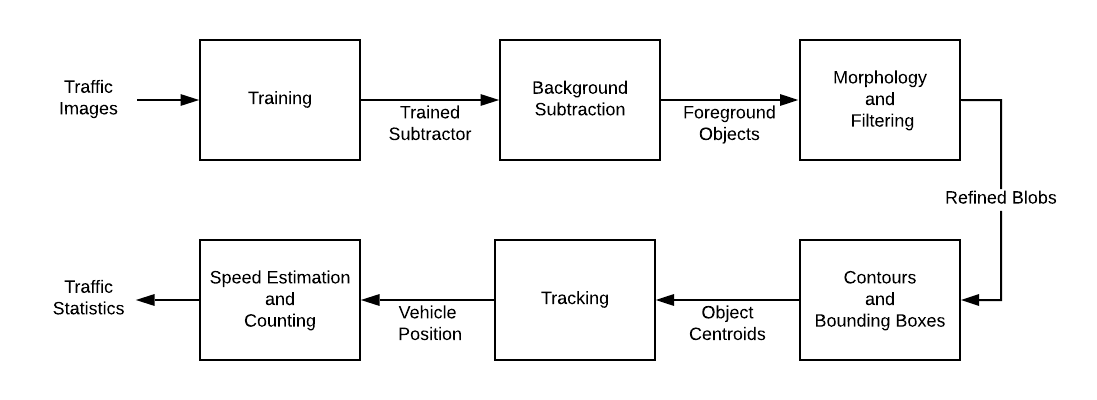
\includegraphics[width=0.9\columnwidth]{design/detection/detection_design}
    \caption{Subprocess that comprise the detection subsystem.}
    \label{fig:detection_design}
\end{figure}



\subsection{Countours and Bounding Boxes}

Contours represent the outline of a foreground object and bounding boxes are the corrected squares that are placed around the polygons that represent an object's outline. These bounding boxes are important for in the tracking of a object.




\subsection{Tracking}

Tracking is follows an objects movement across multiple images. This requires that the object be reidentified in each new image and matched to it's old location.

\subsection{Speed Estimation and Counting}

This subprocess consolidates the efforts of the former ones and convert the information about an objects position into vehicle counts and speeds.


\subsection{Background Subtraction}
\label{subsection:training}

Background subtraction is the process of determining which pixels belong to the background and which are foreground objects. The Gaussian Mixture Model method of clustering (\ref{subsection:mog}) was used to group pixels into foreground and background classes, where the foreground pixel class contains vehicle objects. The background subtractor takes video of the traffic scenario as input and returns a binary output image where all foreground pixels are white and background pixels are black, known as a foreground mask. 

This component of the algorithm was the most computationally expensive but because image processing was required to occur in real-time it was imperative that a fast implementation was used. Fortunately the OpenCV's BackgroundSubtractorMOG2 function \cite{opencv_mog2} is both fast and effective making it a suitable choice for a low power microcontroller. OpenCV's Mixture of Gaussians implementation is based on the the research by Zoran Zivkovic and Ferdinand van der Heijden \cite{zivkovic_pattern_recognition} \cite{zivkovic_heijden_pattern_recognition_letters}.

Figure \ref{fig:example_subtraction} shows the application of the background subtractor on an arbitrary traffic image highlighting its ability to isolate moving objects. Movement changes the value of pixels over a short time scale making it easy for the model to detect them as foreground objects. OpenCV's GMM implementation also allows a third shadow cluster to be created. Where normally a binary output would be generated, with background pixels are black and foreground pixels white, the shadow cluster generates grey pixels with can then be easily thresholded from the image. In Figure \ref{fig:foreground_mask_unfiltered} the grey pixels in and around the white foreground objects are shadows which are removed via thresholding (\ref{subsection:thresholding}).

\subsubsection{Calibration}

OpenCV's Gaussian Mixture Model (GMM) implementation has two important parameters to consider, \emph{history} and \emph{shadows}, where history is an integer and shadows is a Boolean. 

The history parameter determines how many formerly processed images affect the Gaussian Mixture Model, the longer the history the more insensitive the background model becomes to change. For example, if the subtractor's history is 500 and it processes 501 images then the 1st image no longer has influence on the subtractor's models but the 501st does. For a 30fps video 500 images is only about 16 seconds, therefore if a vehicle stops for that long its presence will be completely absorbed into the background cluster. In Figure \ref{fig:cluster_adaptation} the vehicles in the third lane are stationary for sufficiently long to be absorbed into the background by the GMM, this is not an issue as when they move again they are recognized once more. Thus, the history length should be long enough to absorb small but consistent changes in pixel values, like swaying tree branches, into the background but short enough that a slowly moving vehicle registers as a foreground object. 

The shadows parameter tells the model if a cluster for shadows should be specified. In this system's implementation they are set to true as it allows them to be removed from the foreground mask, Figures \ref{fig:foreground_mask_unfiltered} and \ref{fig:thresh_shadow} show their presence and consequent removal via thresholding. 

The subtractor when initialized hasn't had a chance to develop cluster distributions meaning that initially many background pixels are considered foreground pixels. By first processing a few hundred frames of video input the Gaussian Mixture Model distributions can be given time to settle. This \q{training} step should performed before data collection begins to avoid false readings.
 
\begin{figure}[H]
	\centering
	\begin{subfigure}[b]{0.4\linewidth}
        \centering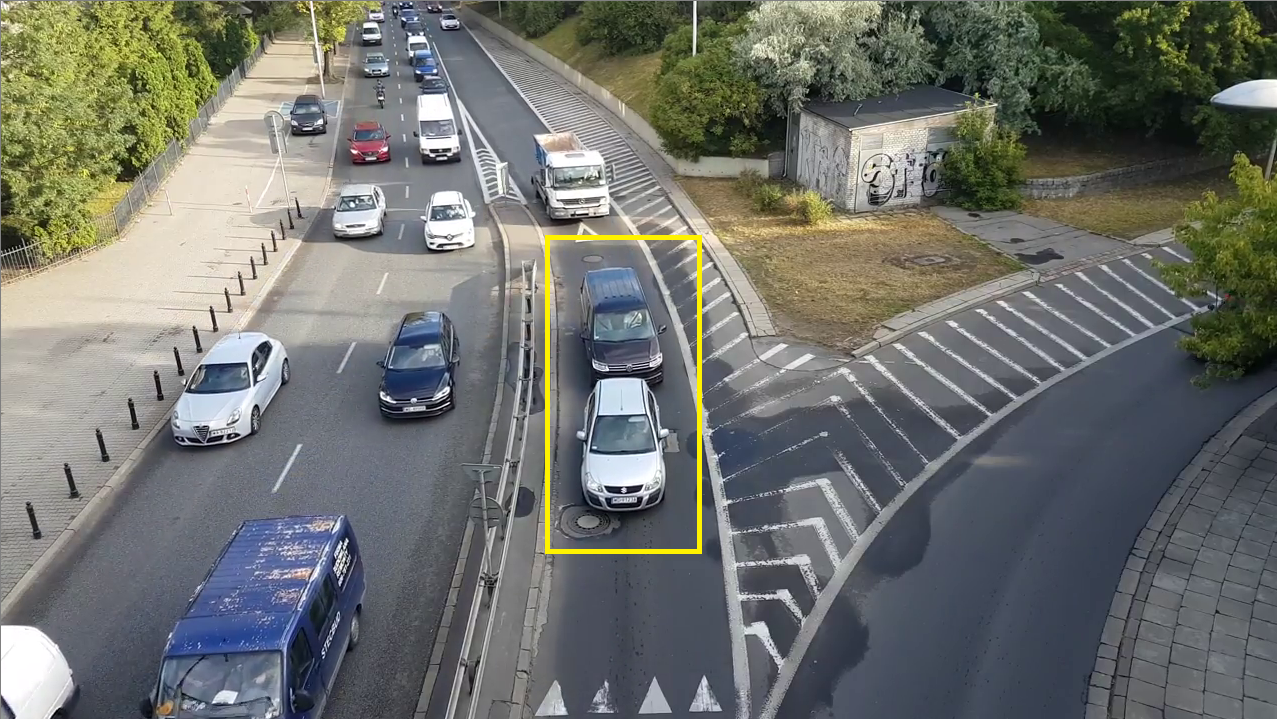
\includegraphics[width = \textwidth]{design/detection/calibration/original}
        \caption{Original Frame - vehicles moving.}
    \end{subfigure}%
    \begin{subfigure}[b]{0.4\linewidth}
        \centering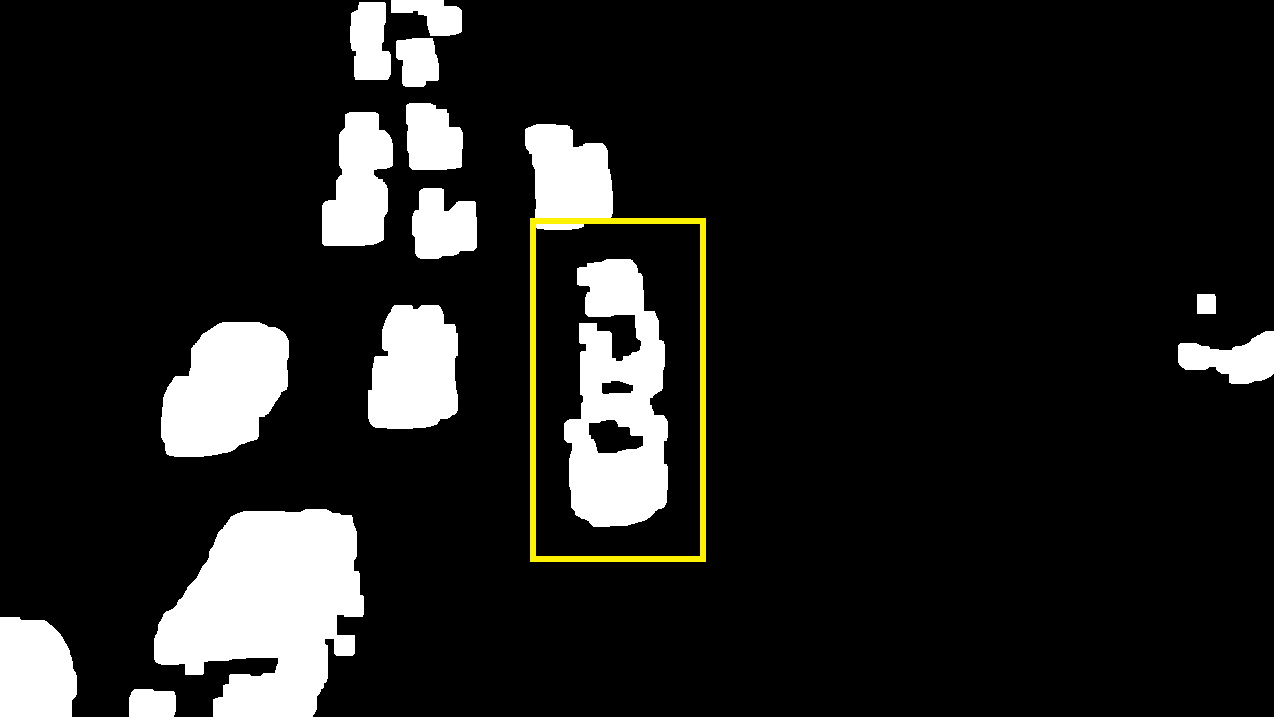
\includegraphics[width = \textwidth]{design/detection/calibration/mask}
        \caption{Foreground Mask - vehicles moving.}
    \end{subfigure}
    \begin{subfigure}[b]{0.4\linewidth}
        \centering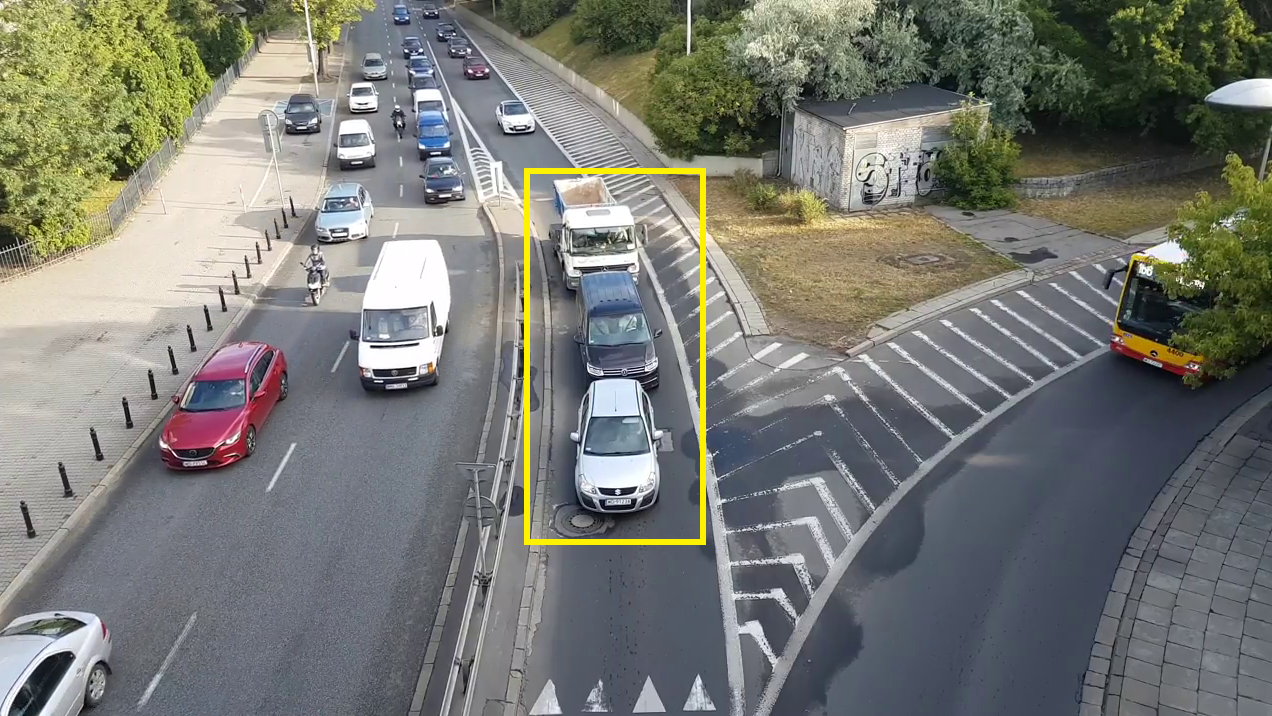
\includegraphics[width = \textwidth]{design/detection/calibration/original_adapted}
        \caption{Original Frame - vehicles stopped.}
    \end{subfigure}%
    	\begin{subfigure}[b]{0.4\linewidth}
        \centering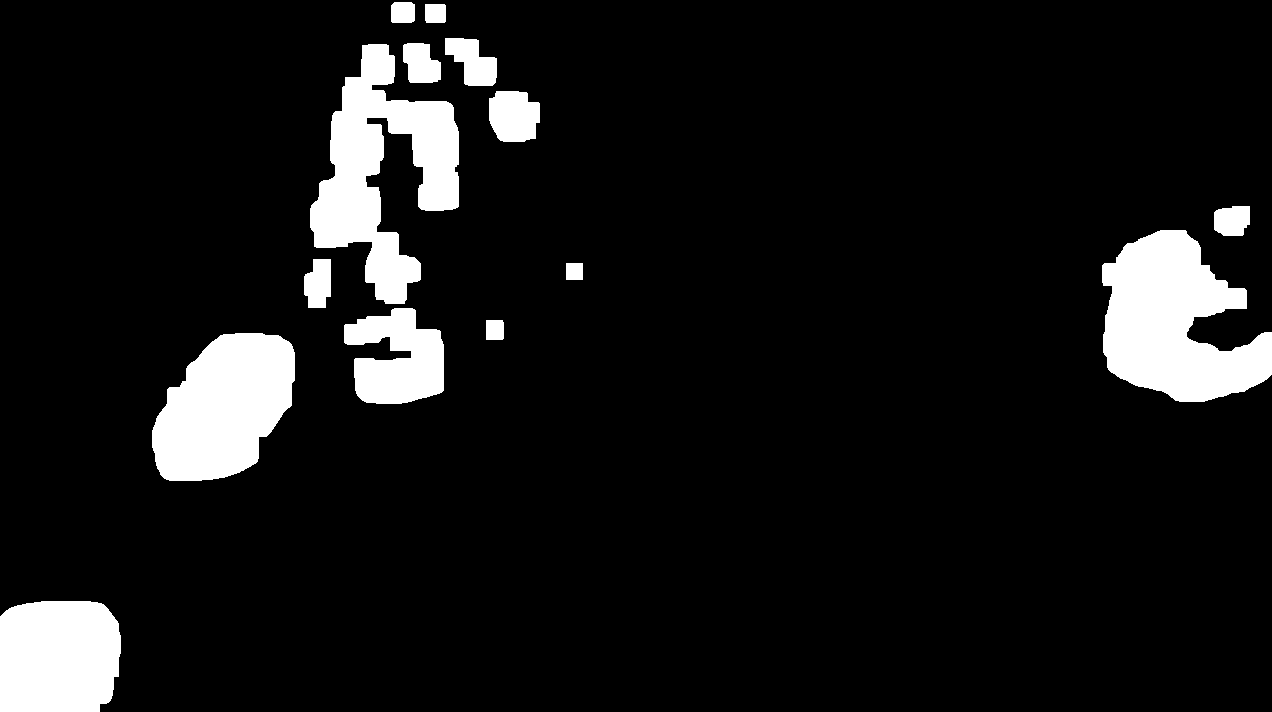
\includegraphics[width = \textwidth]{design/detection/calibration/mask_adapted}
        \caption{Foreground Mask - vehicles stopped.}
    \end{subfigure}
    \caption{Adaptation GMM background cluster. Images by Karol Majek}
    \label{fig:cluster_adaptation}
\end{figure}



\subsection{Morphology and Filtering}

The Morphology and Filtering component of the algorithm takes the foreground mask as input from the background subtractor removing noise and combining foreground objects together that are fractured. 

\subsubsection{Median Filtering}

Often salt and pepper noise is generated by the subtraction process due to lighting changes, camera instability and non-target object movement like trees and humans. By applying a median filter (\ref{subsubsection:median_filter}) this noise can be removed. Figure \ref{fig:foreground_mask_filtered} shows the effect of applying a median filter to remove noise from a foreground mask. It's important to remove this noise because it's doesn't represent a vehicle and it may lead to incorrect data collection output. The OpenCV method medianBlur() was used to implement this functionality.

\subsubsection{Morphology}

Vehicles sometimes do not form a connected-component of 1-pixels in the foreground mask. The GMM clusters pixels on their colour so any parts of a vehicle that appear similar in colour to the background distribution, which is most often the colour of the road, are classified as background pixels. Car windows in particular are incorrectly classified as background pixels because they reflect light from the road. This phenomenon can cause a single vehicle to be represented in the foreground mask as a number of disconnect-components. This is bad as it appears to other parts of the algorithm that there are more vehicles than one. Figure \ref{fig:example_subtraction} shows an example of a single vehicle generating many distinct blobs. By applying morphology to the foreground mask these blobs can be recombined into a single entity.

To recombine fractured blobs a morphological closing and dilation (\ref{section:morphology}) are performed, Figure \ref{fig:foreground_mask_morphed} shows an example of blob recombination. The OpenCV function morphologyEx() was used to perform these operations. The selection of structuring element shapes, size and number of iterations is dependent on the specific traffic scene presented and requires considerable calibration. 

\subsubsection{Calibration}

Usually at least one region of the foreground mask has more correct pixel clustering than another, this is often a consequence of the lighting in that region of the input images. When calibrating the morphological operations the area to focus on improving is this region. In a situations where the camera perspective is not directly above the traffic setting looking down it's not possible to improve all regions of the image as the perceived size of the vehicles changes throughout the image. Hence, the morphological structuring should be selected for a specific region of improvement. In situations where the camera perspective is perpendicular to vehicle movement, the structuring element selection will work for the entire image as vehicle scale doesn't change. Figure \ref{fig:perspective} illustrates the difference in these perspectives.

\begin{figure}[h]
    \centering
     \begin{subfigure}[b]{0.45\textwidth}
        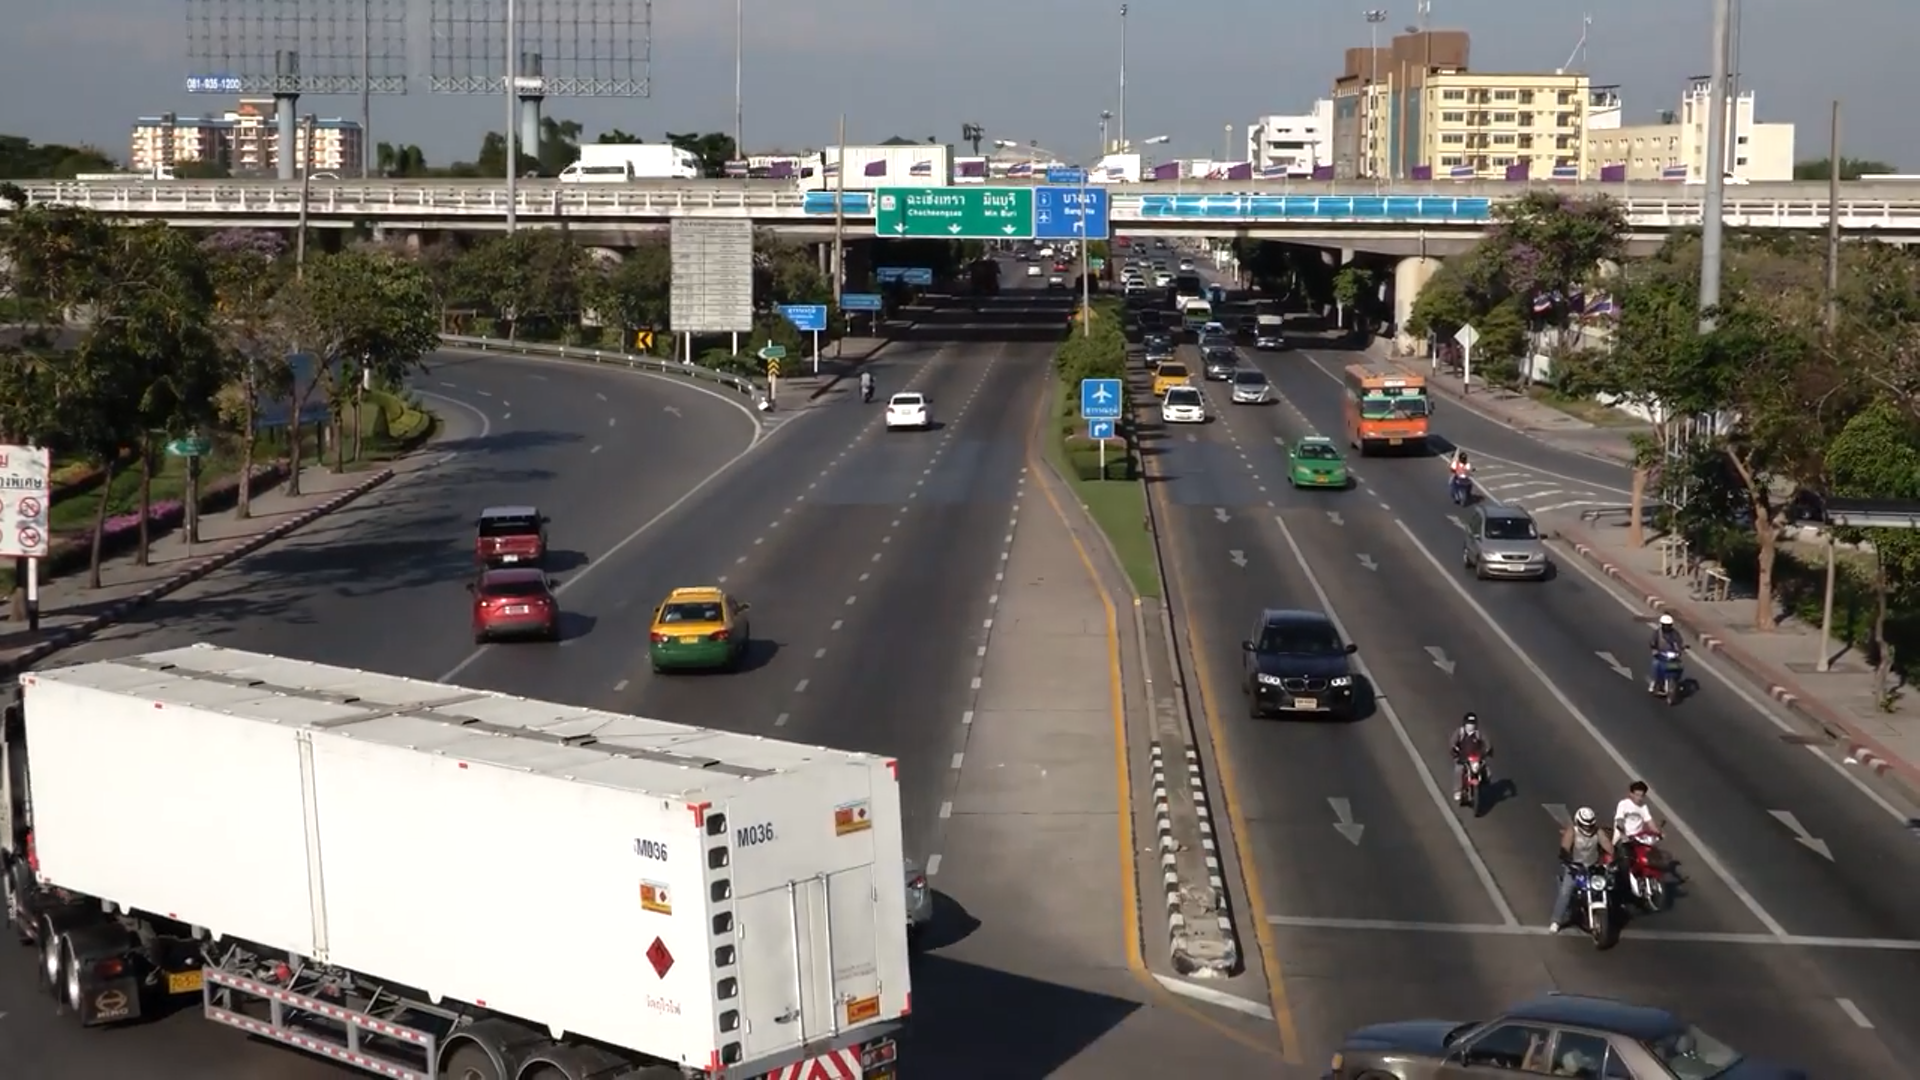
\includegraphics[width=\textwidth]{design/detection/morphology/perspectiveA}
	\captionsetup{format = hang}
        \caption{Changing vehicle scale perspective.}
    \end{subfigure} 
    \begin{subfigure}[b]{0.45\textwidth}
        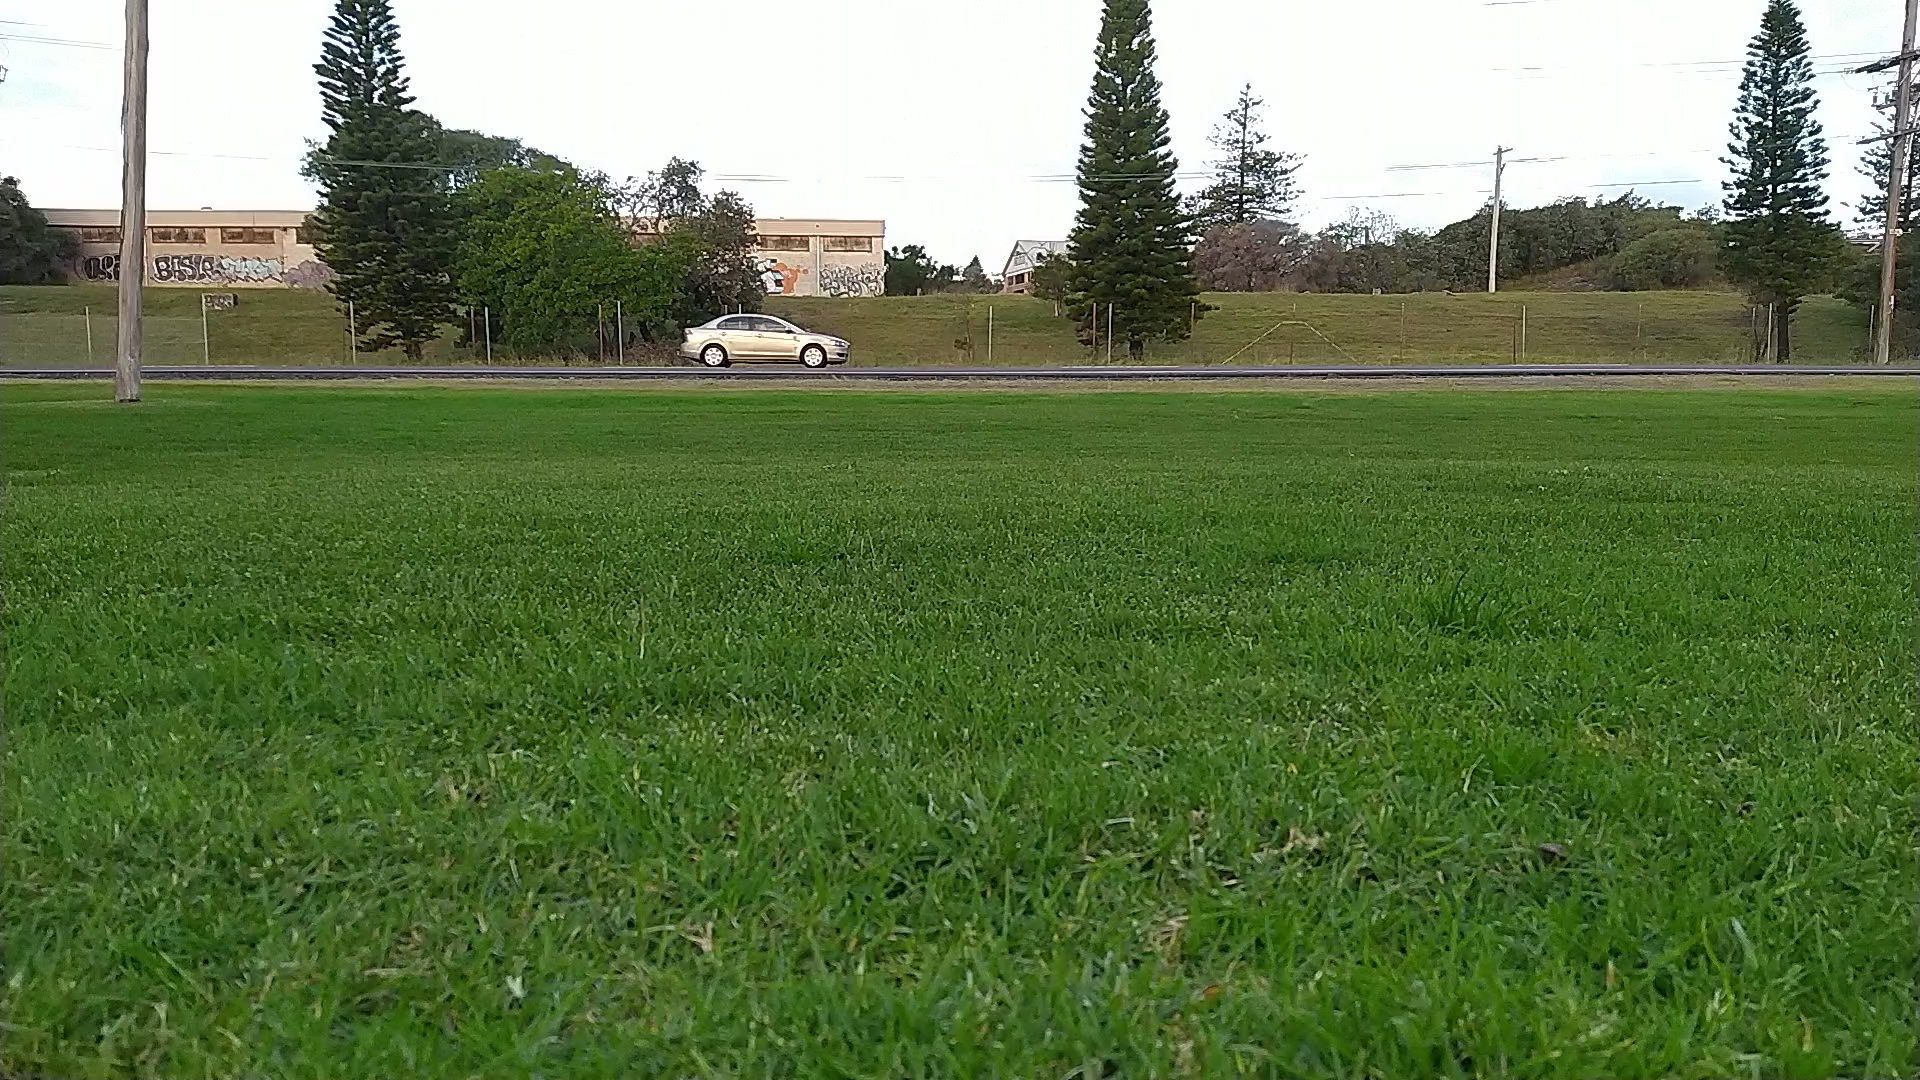
\includegraphics[width=\textwidth]{design/detection/morphology/perspectiveB}	
	\captionsetup{format = hang}
        \caption{Fixed vehicle scale perspective.}
    \end{subfigure}
    \captionsetup{format = hang}
    \caption{Comparison of camera perspective and its affect on vehicle scale.}
    \label{fig:perspective}
\end{figure}

Morphological operations can be computationally expensive depending on the size of the structuring element and number of iterations performed. In order to maintain real-time image processing minimising these factors for each traffic scenario is important. Figure \ref{fig:morph_testing} shows the comparative performance of three structuring element shapes on the same foreground mask for a 7x7 element size and varying iterations. Visual analysis of each outcome showed that the rectangular element performed for 3 iterations gave the best result because it generated the best recombination of blobs. Figure \ref{fig:compare_closure} shows an example blob recombination, in this case the rectangular structuring element successfully recombined the blob where the elliptical element could not.

\begin{figure}[H]
    \centering
    \begin{subfigure}[b]{0.45\textwidth}
        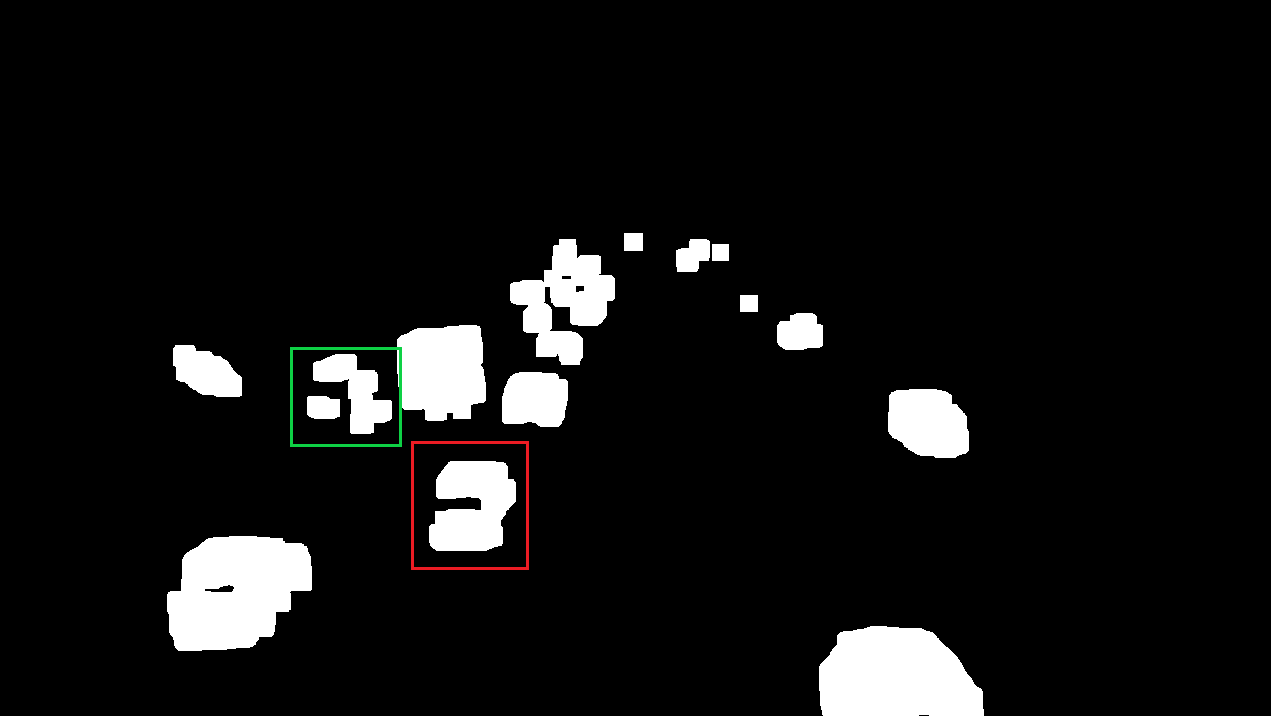
\includegraphics[width=\textwidth]{design/detection/calibration/rect_3_edit}
        \caption{Closure with rectangle.}
    \end{subfigure}
    \begin{subfigure}[b]{0.45\textwidth}
        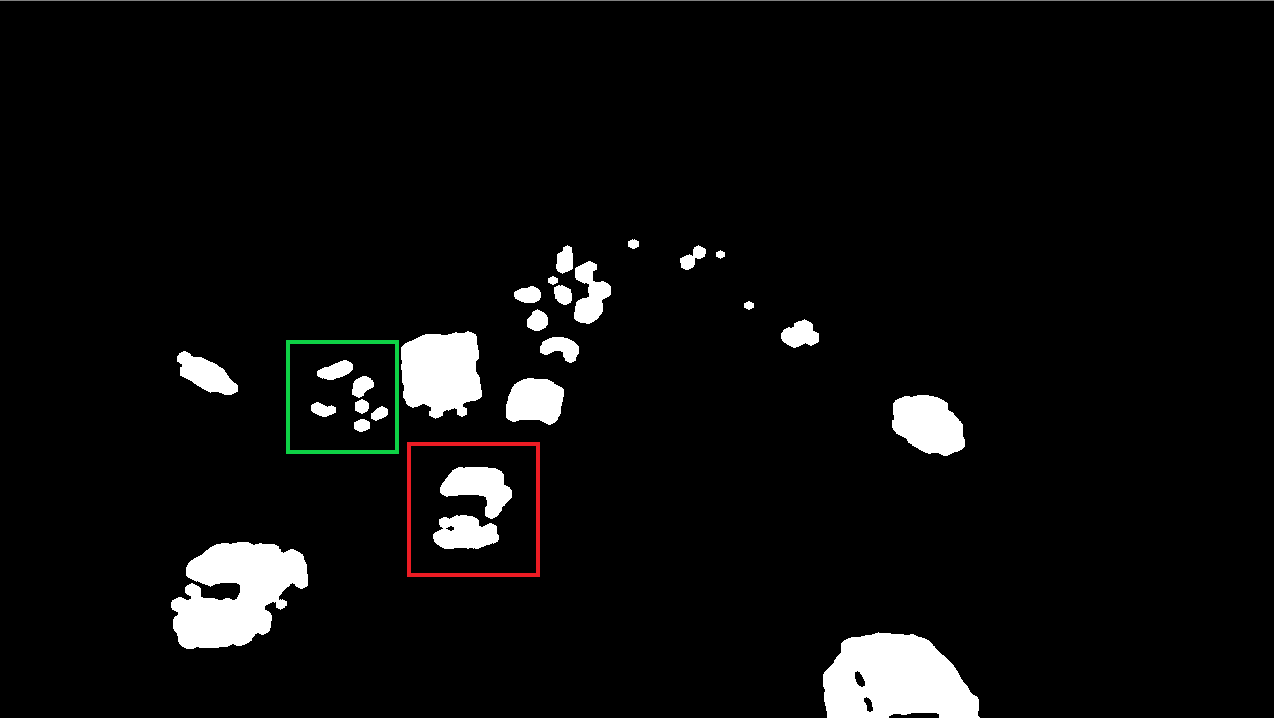
\includegraphics[width=\textwidth]{design/detection/calibration/ellipse_3_edit}
        \caption{Closure with ellipse.}
    \end{subfigure}
    \captionsetup{format = hang}
    \caption{Comparison of morphological closure using a 7x7 rectangular and elliptical structuring element for 3 iterations.}
    \label{fig:compare_closure}
\end{figure}


\begin{figure}[H]
    \begin{tabular}{
        >{\centering\arraybackslash}m{0.4cm}
        >{\centering\arraybackslash}m{4.5cm}
        >{\centering\arraybackslash}m{4.5cm}
        >{\centering\arraybackslash}m{4.5cm}}
          & Ellipse & Cross & Rectangle \\
        1 
        &
        \begin{subfigure}[b]{0.3\textwidth}
            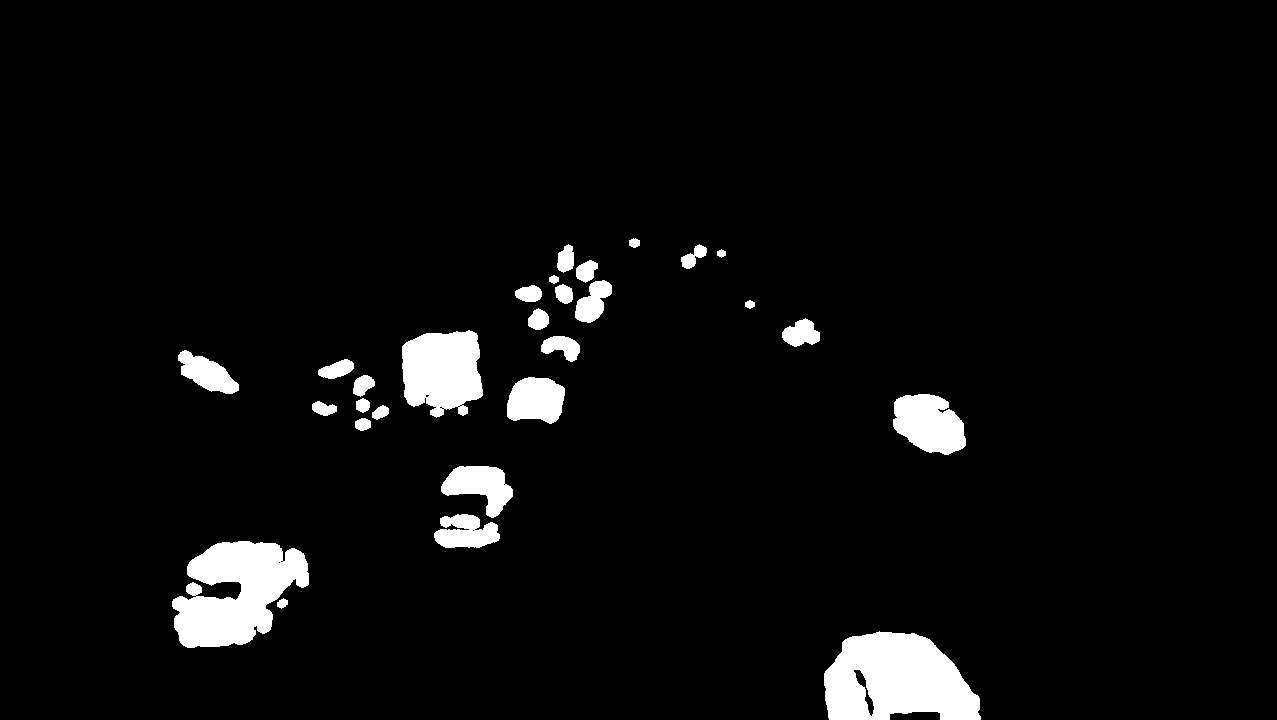
\includegraphics[width=\textwidth]{design/detection/morphology/ellipse_1}
            % \captionsetup{format = hang}
        \end{subfigure} &
        \begin{subfigure}[b]{0.3\textwidth}
            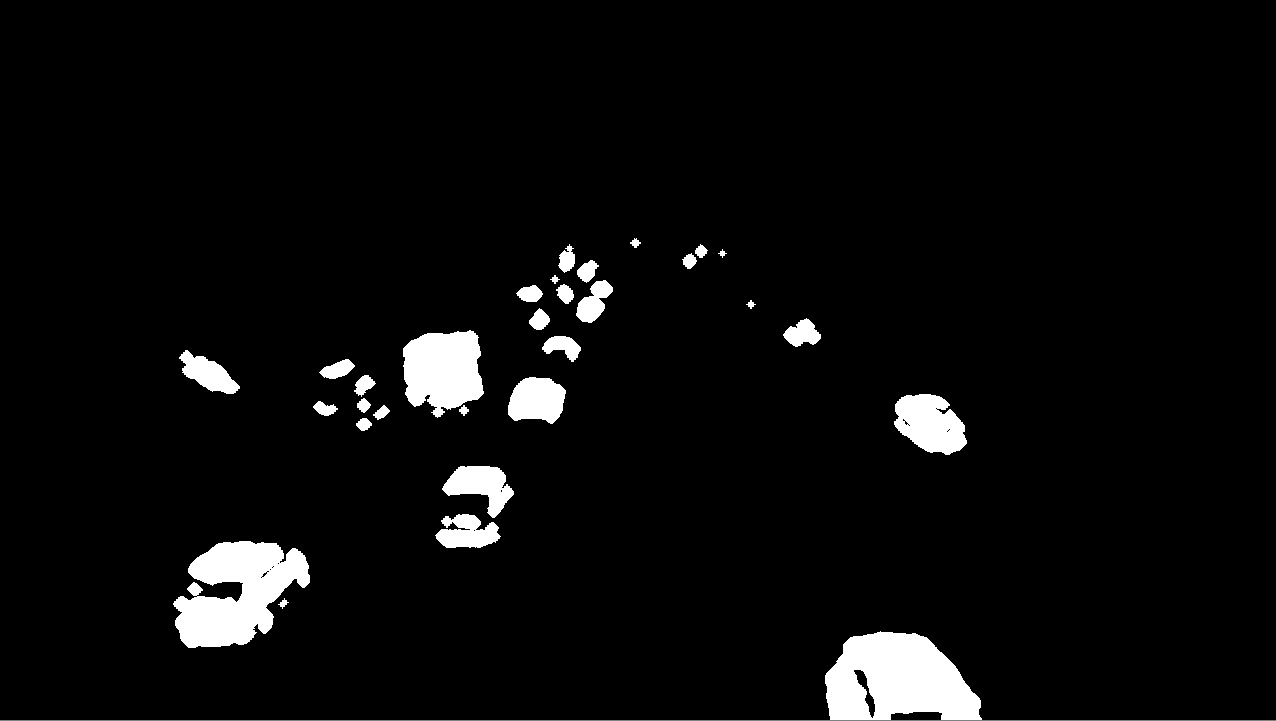
\includegraphics[width=\textwidth]{design/detection/morphology/cross_1}
            % \captionsetup{format = hang}
        \end{subfigure} &
        \begin{subfigure}[b]{0.3\textwidth}
            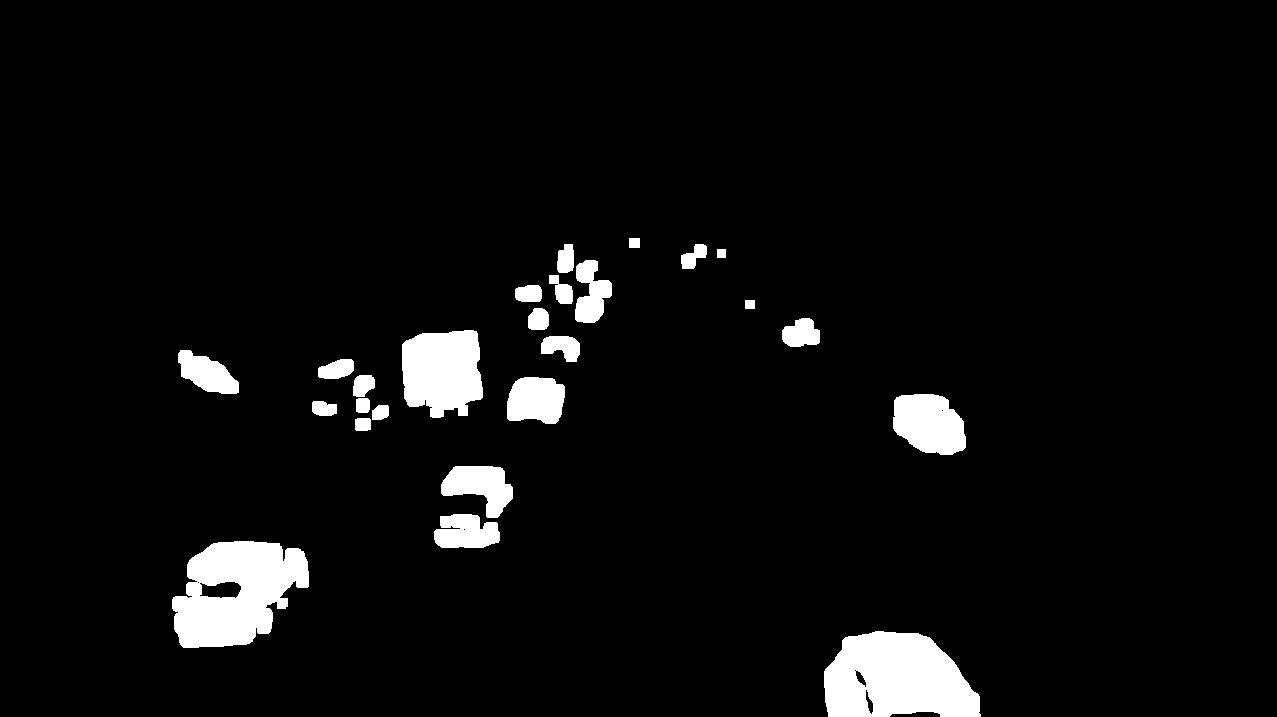
\includegraphics[width=\textwidth]{design/detection/morphology/rect_1}
            % \captionsetup{format = hang}
        \end{subfigure} \\
        3 &
        \begin{subfigure}[b]{0.3\textwidth}
            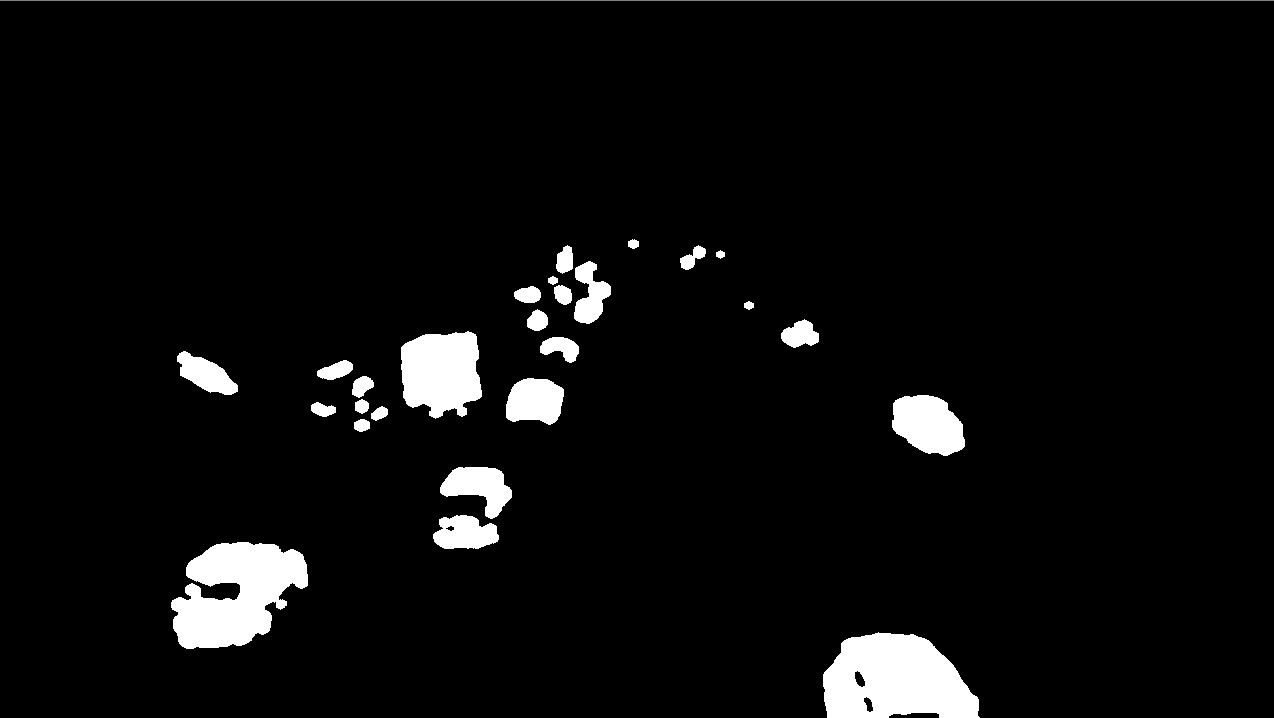
\includegraphics[width=\textwidth]{design/detection/morphology/ellipse_3}
            % \captionsetup{format = hang}
        \end{subfigure} &
        \begin{subfigure}[b]{0.3\textwidth}
            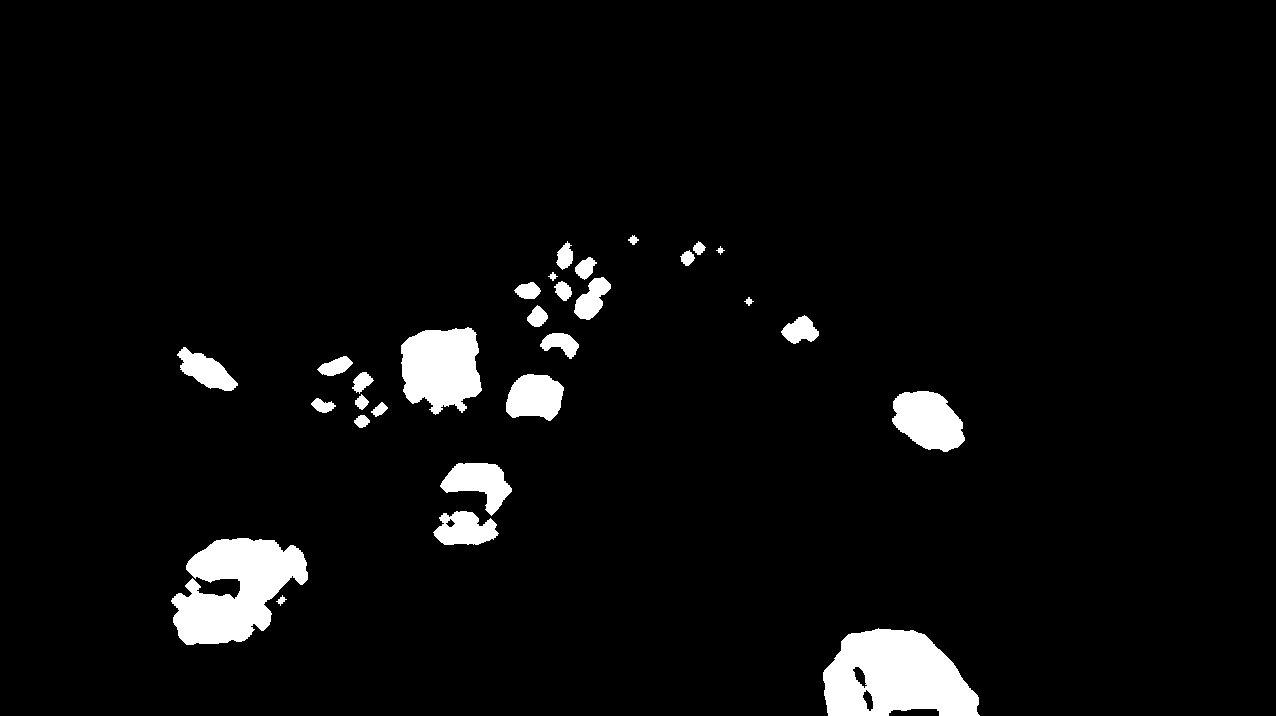
\includegraphics[width=\textwidth]{design/detection/morphology/cross_3}
            % \captionsetup{format = hang}
        \end{subfigure} &
        \begin{subfigure}[b]{0.3\textwidth}
            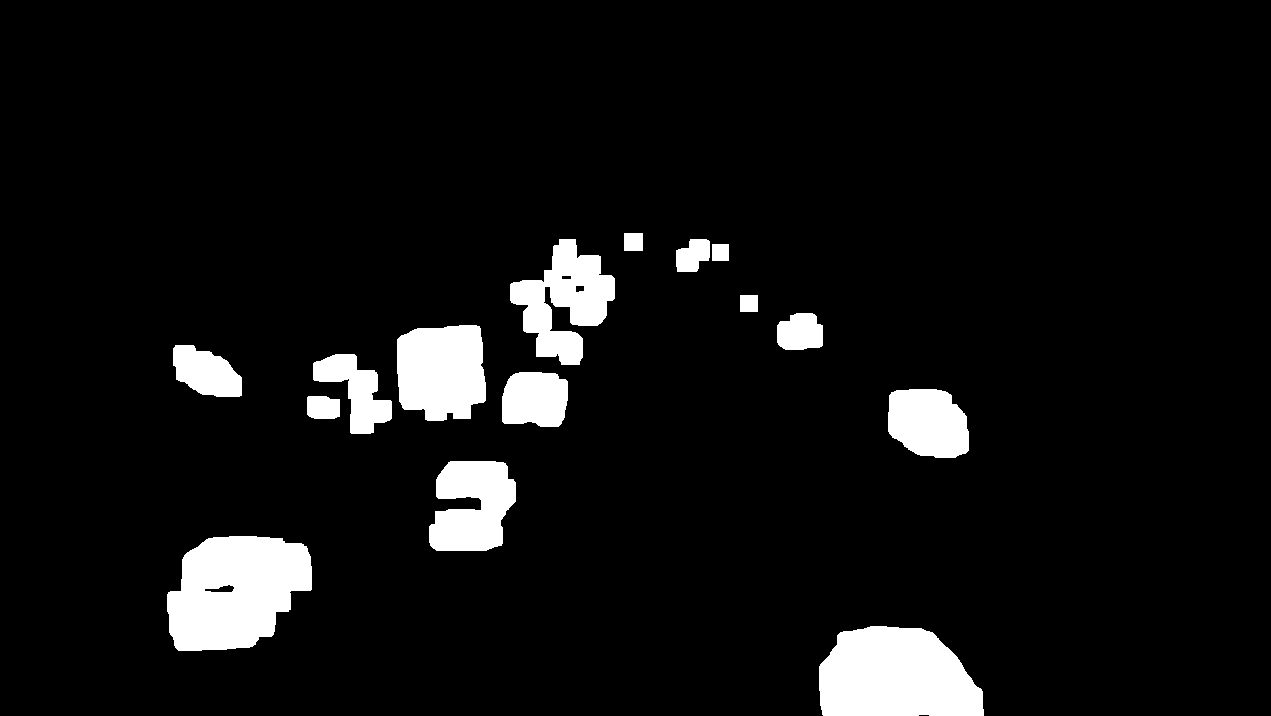
\includegraphics[width=\textwidth]{design/detection/morphology/rect_3}
            % \captionsetup{format = hang}
        \end{subfigure} \\
        5 &
        \begin{subfigure}[b]{0.3\textwidth}
            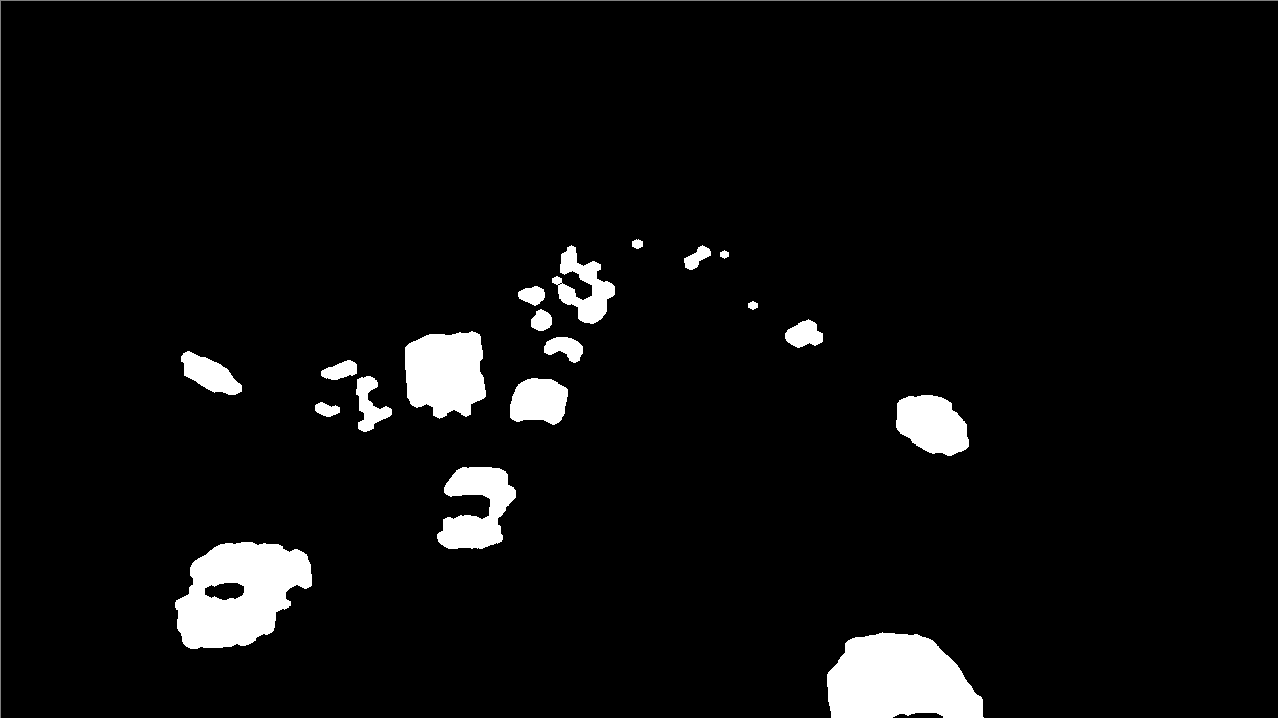
\includegraphics[width=\textwidth]{design/detection/morphology/ellipse_5}
            % \captionsetup{format = hang}
        \end{subfigure} &
        \begin{subfigure}[b]{0.3\textwidth}
            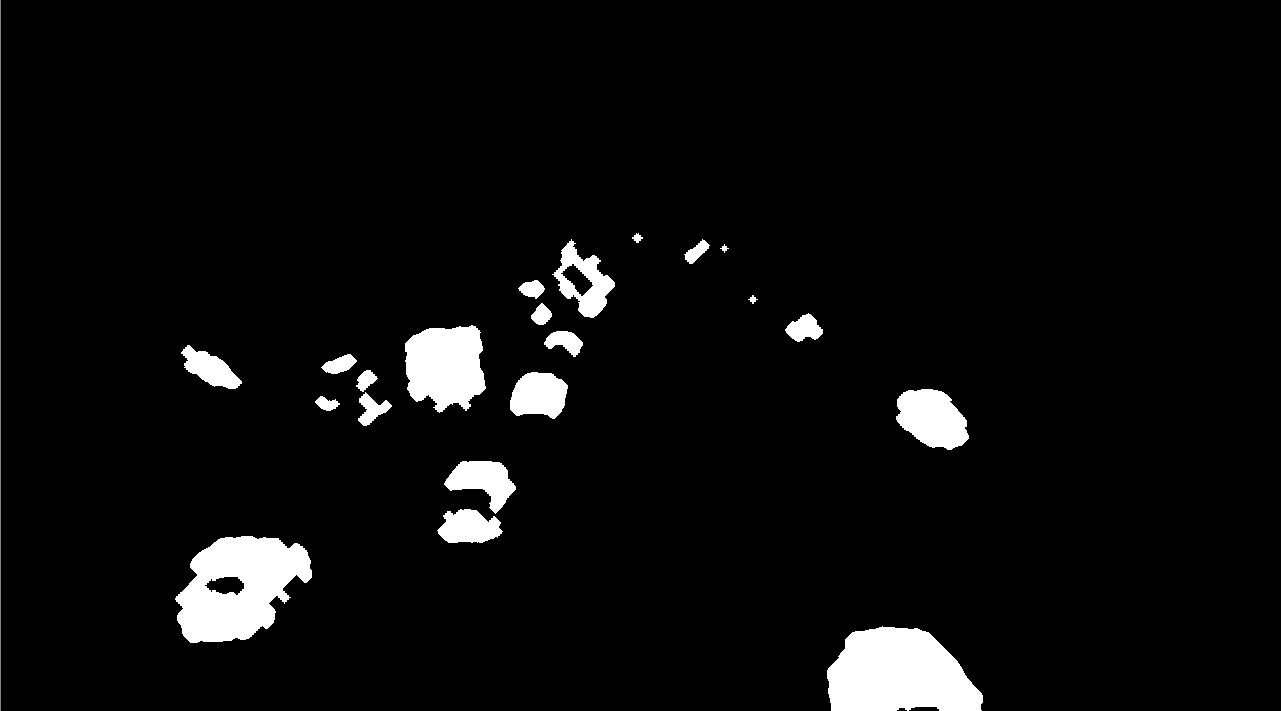
\includegraphics[width=\textwidth]{design/detection/morphology/cross_5}
            % \captionsetup{format = hang}
        \end{subfigure} &
        \begin{subfigure}[b]{0.3\textwidth}
            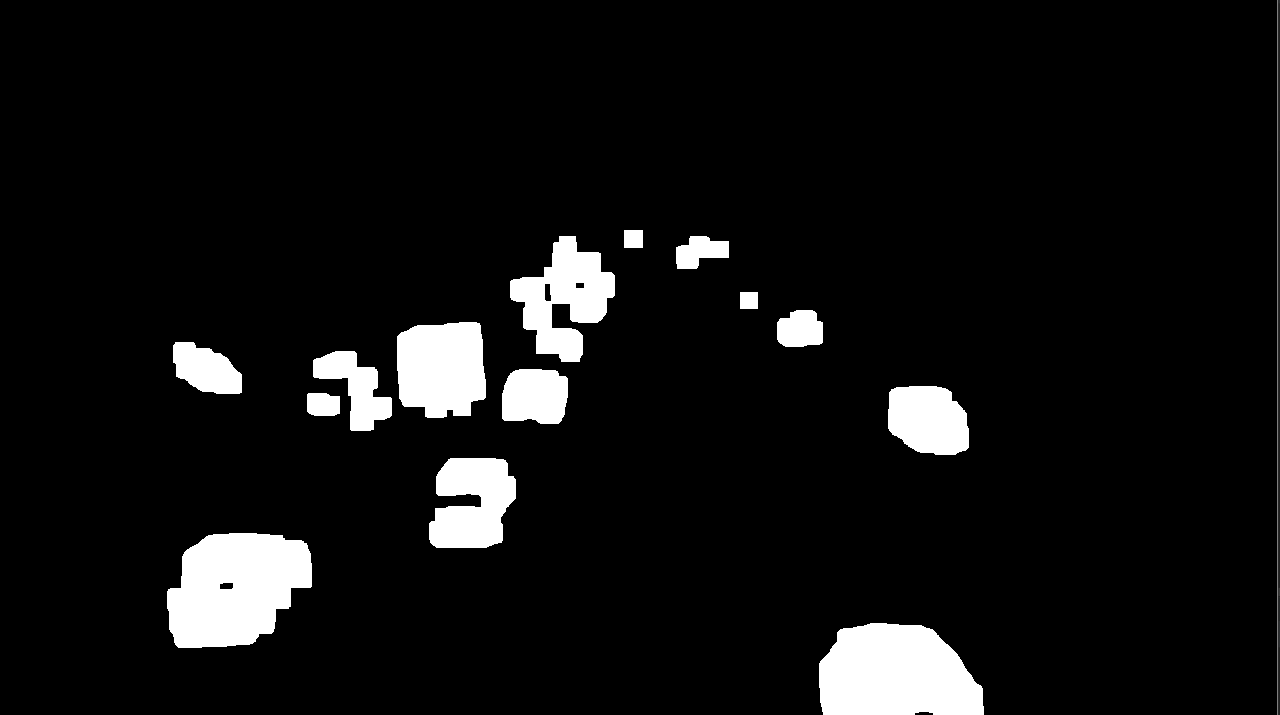
\includegraphics[width=\textwidth]{design/detection/morphology/rect_5}
            % \captionsetup{format = hang}
        \end{subfigure} \\
    \end{tabular}
    \captionsetup{format = hang}
    \caption{Morphological closing using different 7x7 structuring elements and iterations.}
    \label{fig:morph_testing}
\end{figure}

\subsection{Calibration}

It is unfortunate but neccessary that for this method of vehicle classification that for each different location and camera angle an element of calibration is required to obtain best results. This is a function of the size of vehicles in the camera frame and the lighting conditions at the location. Presently these factors are compensated for by manually calibrating the morphological operations and areas of interest for counting and speed measurement. 

\subsubsection{Calibrating Morphological Operations}

To find the optimal morphological structuring element shape and size, and the number of iterations of closing and dilation to perform for the setting in Figure \ref{fig:original_frame} a visual analysis of the effect of a number of settings was performed. For example Figure \ref{fig:morph_testing} show the result of a morphological closure to the output of the background subtractor using different structuring element shapes and closure iterations. 7x7 was formerly settled on as the structuring element size for it produced not too much nor too little effect on the foreground objects. In the visual analysis you seek the result that has converted the most fractured vehicle masks into a single closed contour wit the least iteration, hence for this particular example the optimal morphological closure parameters were a rectangular structuring element with 3 iterations. In Figure \ref{fig:compare_closure} the highlighted shapes have found closure and so will be counted as a single entity in the contouring process.


\begin{figure}[htbp]
    \centering
    \begin{subfigure}[b]{0.42\textwidth}
        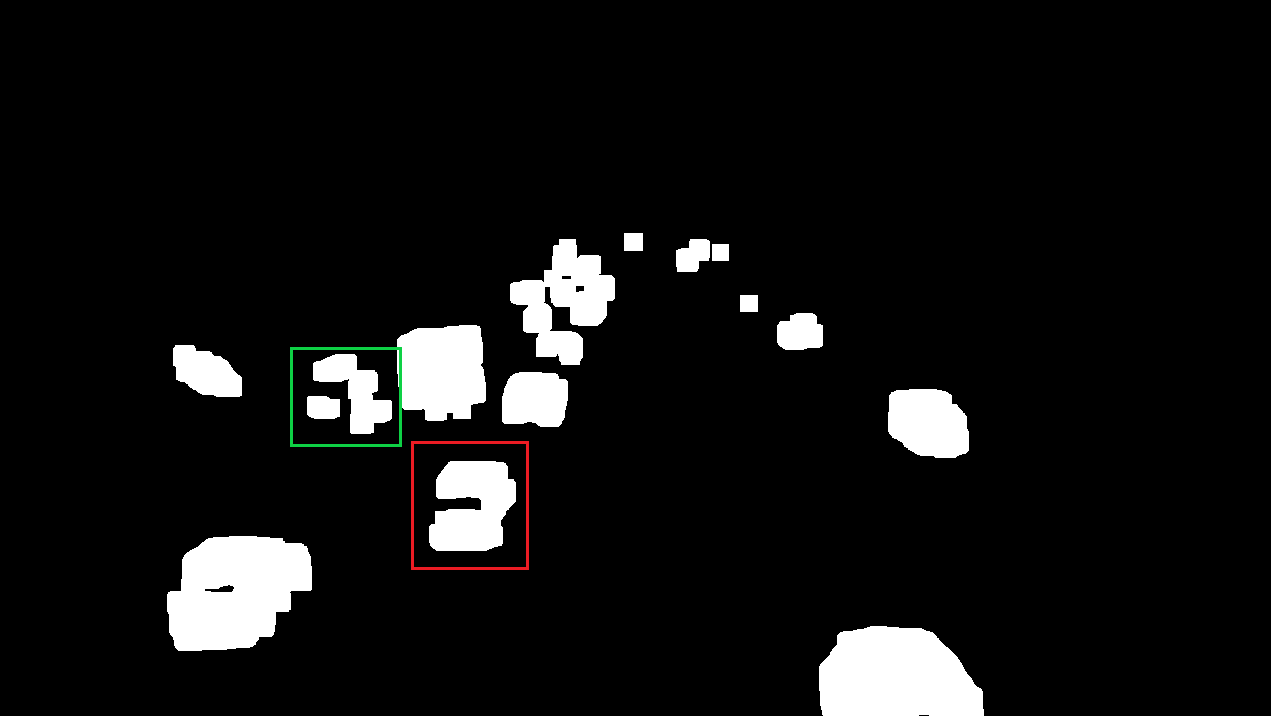
\includegraphics[width=\textwidth]{design/detection/calibration/rect_3_edit}
        \captionsetup{format = hang}
        \caption{Rectangular structuring element closure}
    \end{subfigure}
    \begin{subfigure}[b]{0.42\textwidth}
        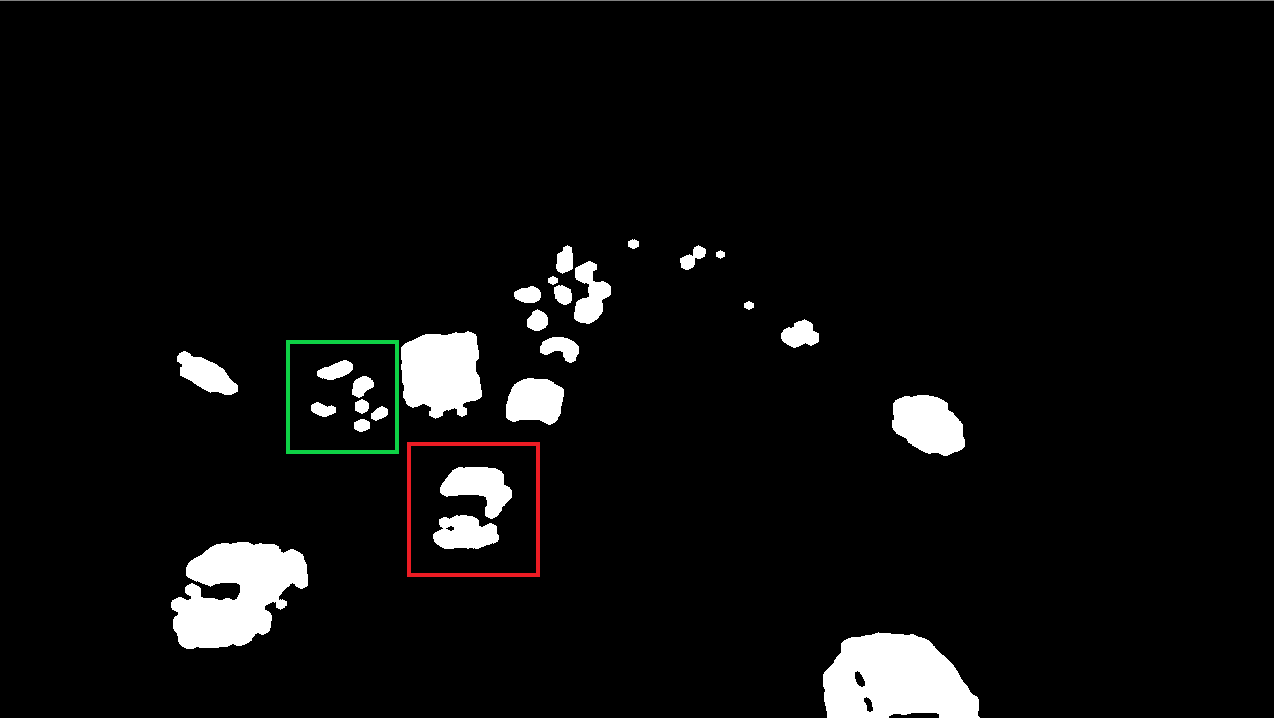
\includegraphics[width=\textwidth]{design/detection/calibration/ellipse_3_edit}
        \captionsetup{format = hang}
        \caption{Elliptical structuring element closure}
    \end{subfigure}
    \captionsetup{format = hang}
    \caption{Comparison of morphological closure using a 7x7 rectangular and elliptical structuring element for 3 iterations.}
    \label{fig:compare_closure}
\end{figure}


\begin{figure*}[htbp]
    \begin{tabular}{
        >{\centering\arraybackslash}m{0.4cm}
        >{\centering\arraybackslash}m{4.5cm}
        >{\centering\arraybackslash}m{4.5cm}
        >{\centering\arraybackslash}m{4.5cm}}
          & Ellipse & Cross & Rectangle \\
        1 
        &
        \begin{subfigure}[b]{0.3\textwidth}
            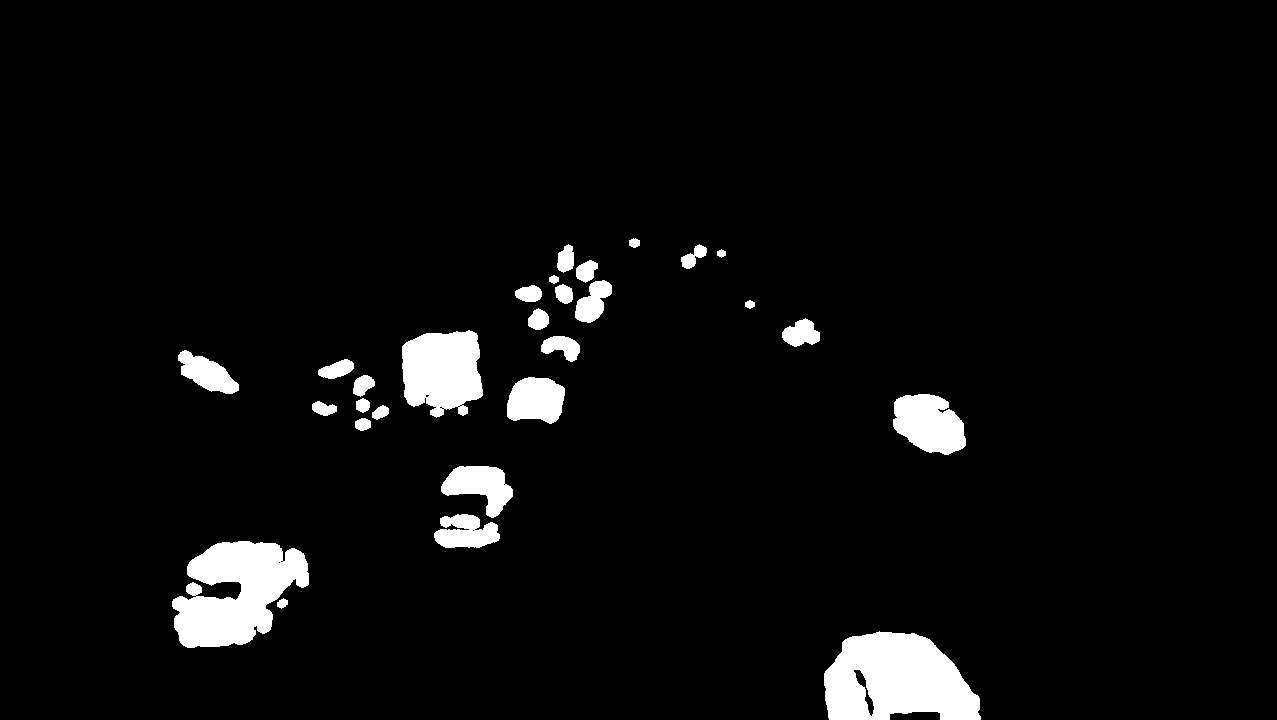
\includegraphics[width=\textwidth]{design/detection/morphology/ellipse_1}
            % \captionsetup{format = hang}
        \end{subfigure} &
        \begin{subfigure}[b]{0.3\textwidth}
            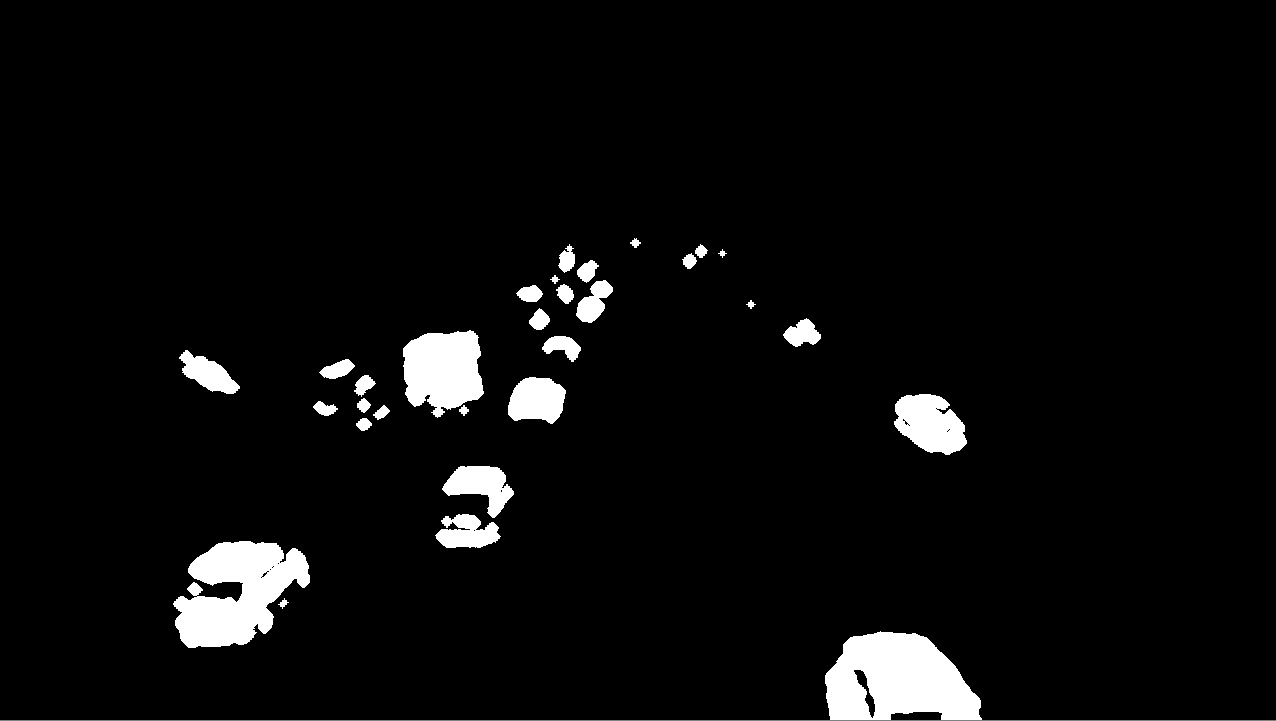
\includegraphics[width=\textwidth]{design/detection/morphology/cross_1}
            % \captionsetup{format = hang}
        \end{subfigure} &
        \begin{subfigure}[b]{0.3\textwidth}
            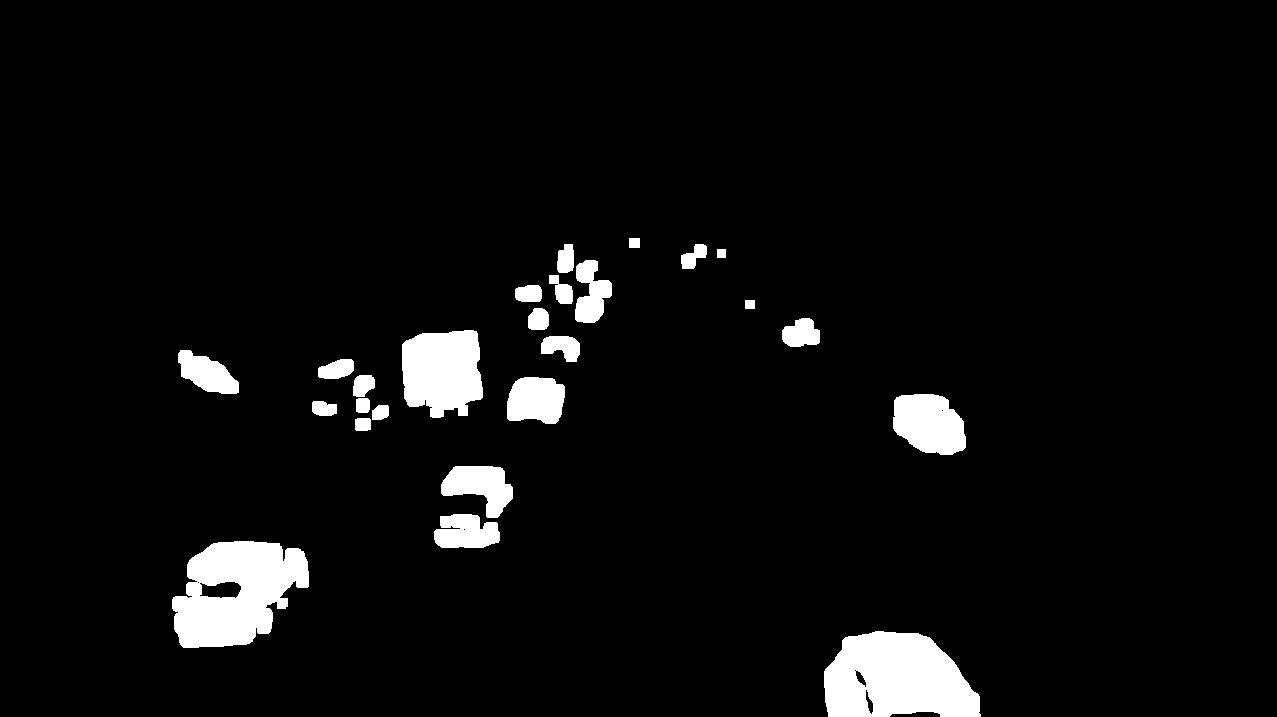
\includegraphics[width=\textwidth]{design/detection/morphology/rect_1}
            % \captionsetup{format = hang}
        \end{subfigure} \\
        3 &
        \begin{subfigure}[b]{0.3\textwidth}
            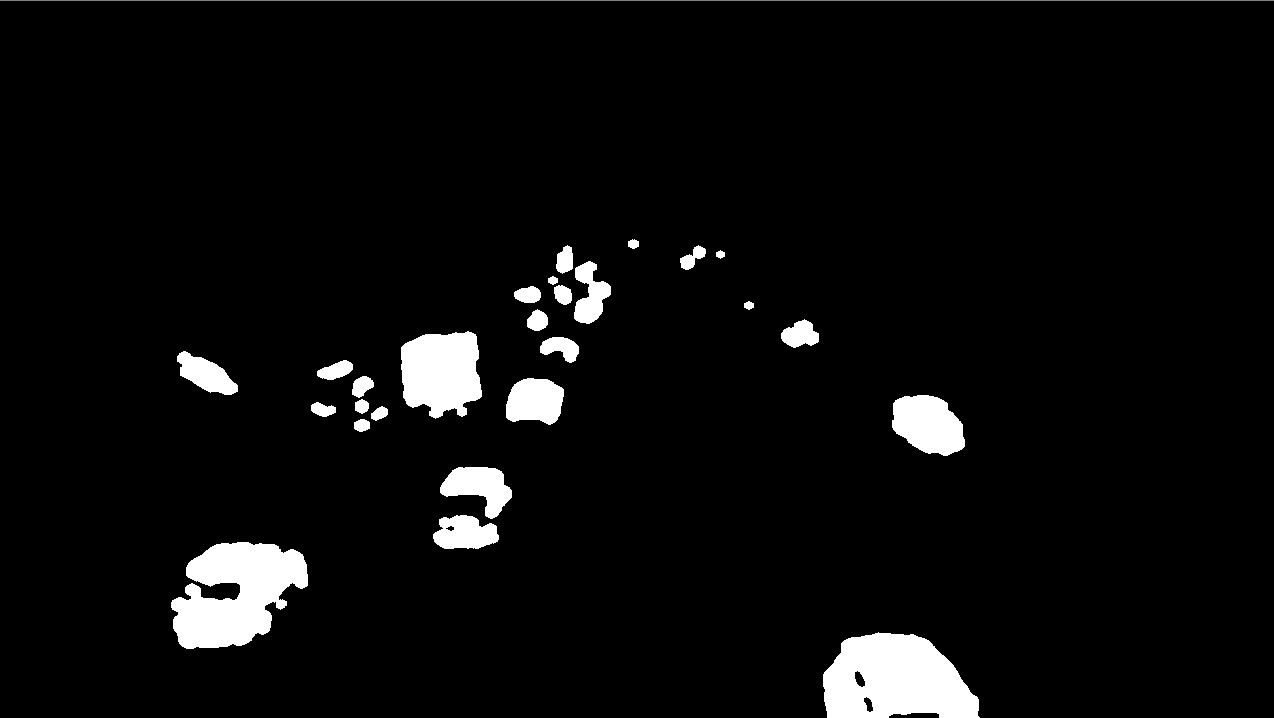
\includegraphics[width=\textwidth]{design/detection/morphology/ellipse_3}
            % \captionsetup{format = hang}
        \end{subfigure} &
        \begin{subfigure}[b]{0.3\textwidth}
            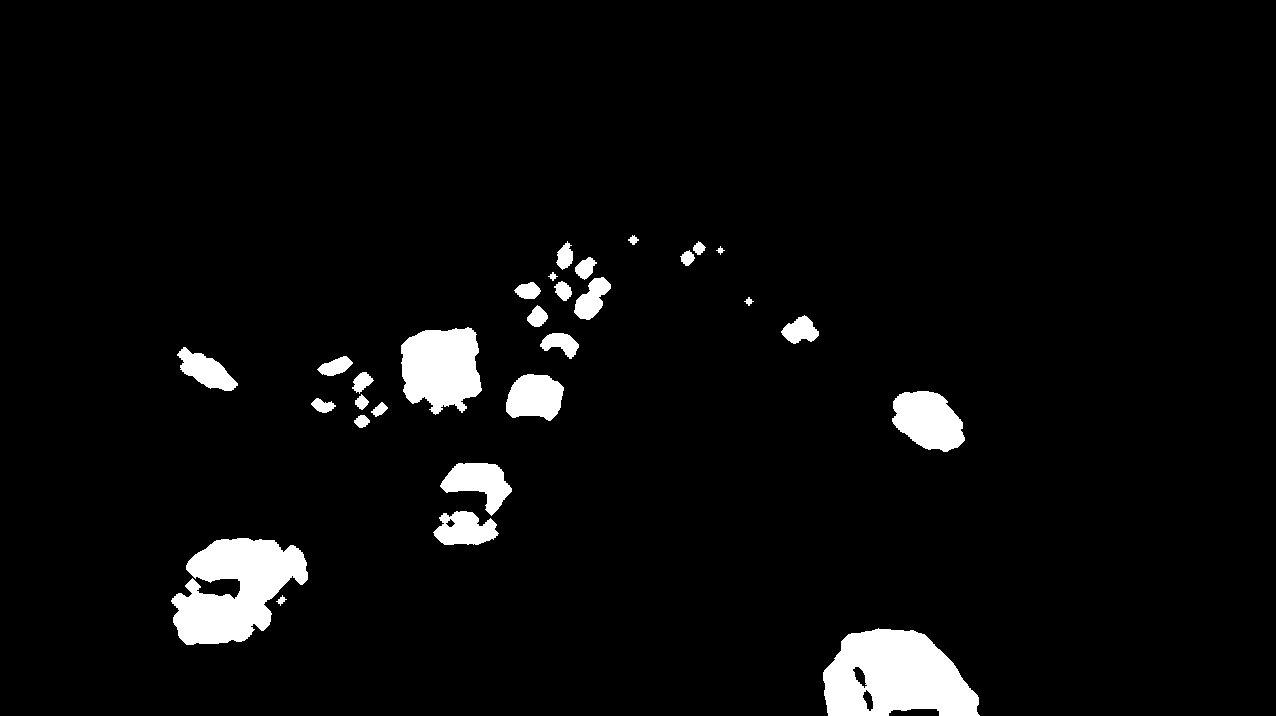
\includegraphics[width=\textwidth]{design/detection/morphology/cross_3}
            % \captionsetup{format = hang}
        \end{subfigure} &
        \begin{subfigure}[b]{0.3\textwidth}
            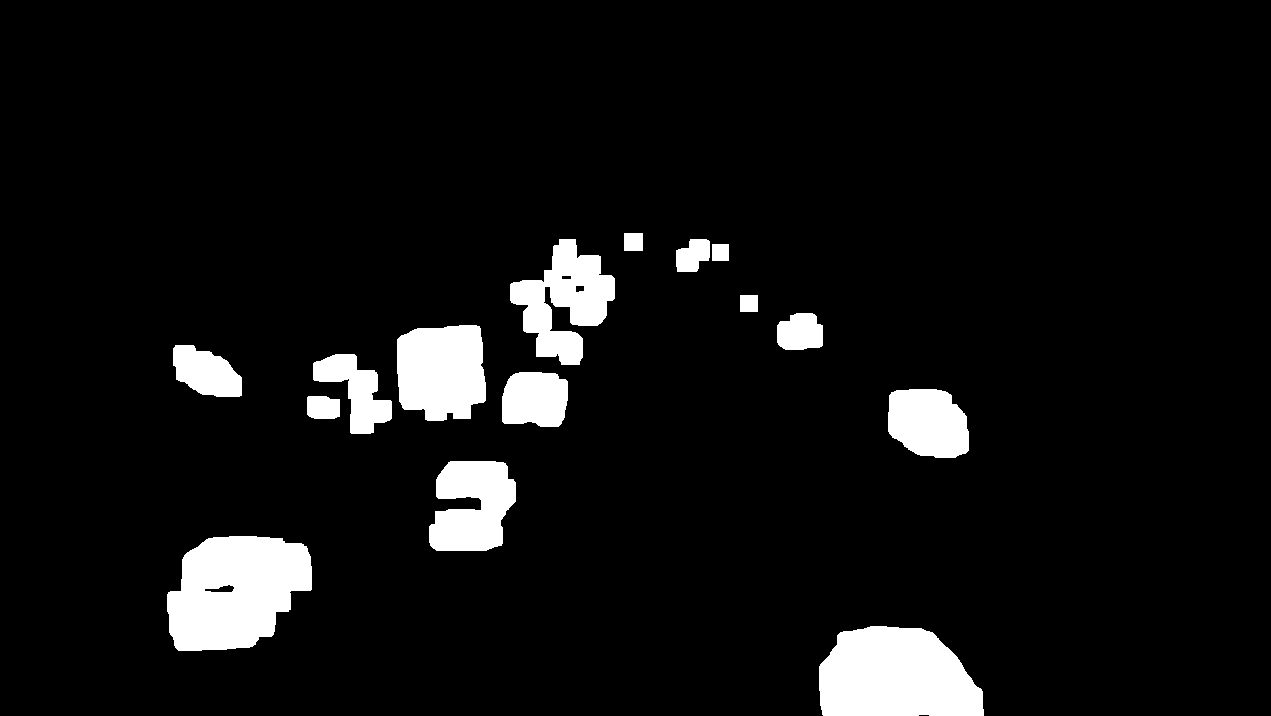
\includegraphics[width=\textwidth]{design/detection/morphology/rect_3}
            % \captionsetup{format = hang}
        \end{subfigure} \\
        5 &
        \begin{subfigure}[b]{0.3\textwidth}
            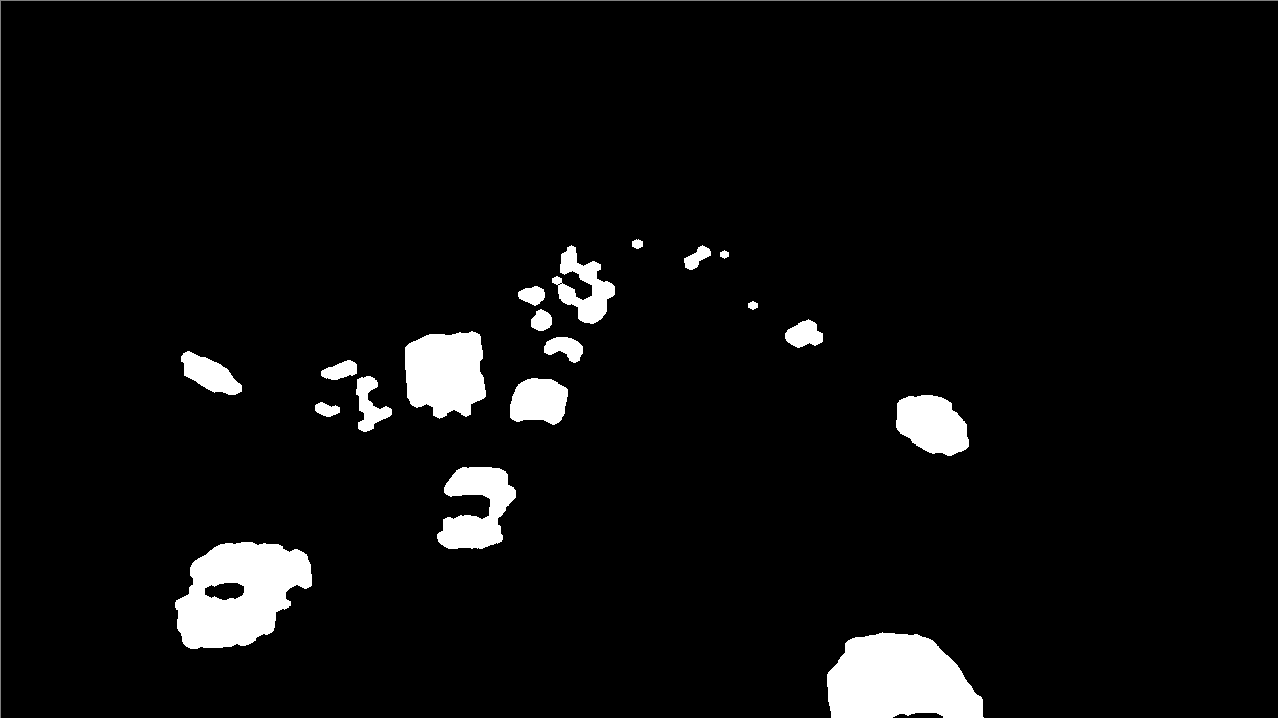
\includegraphics[width=\textwidth]{design/detection/morphology/ellipse_5}
            % \captionsetup{format = hang}
        \end{subfigure} &
        \begin{subfigure}[b]{0.3\textwidth}
            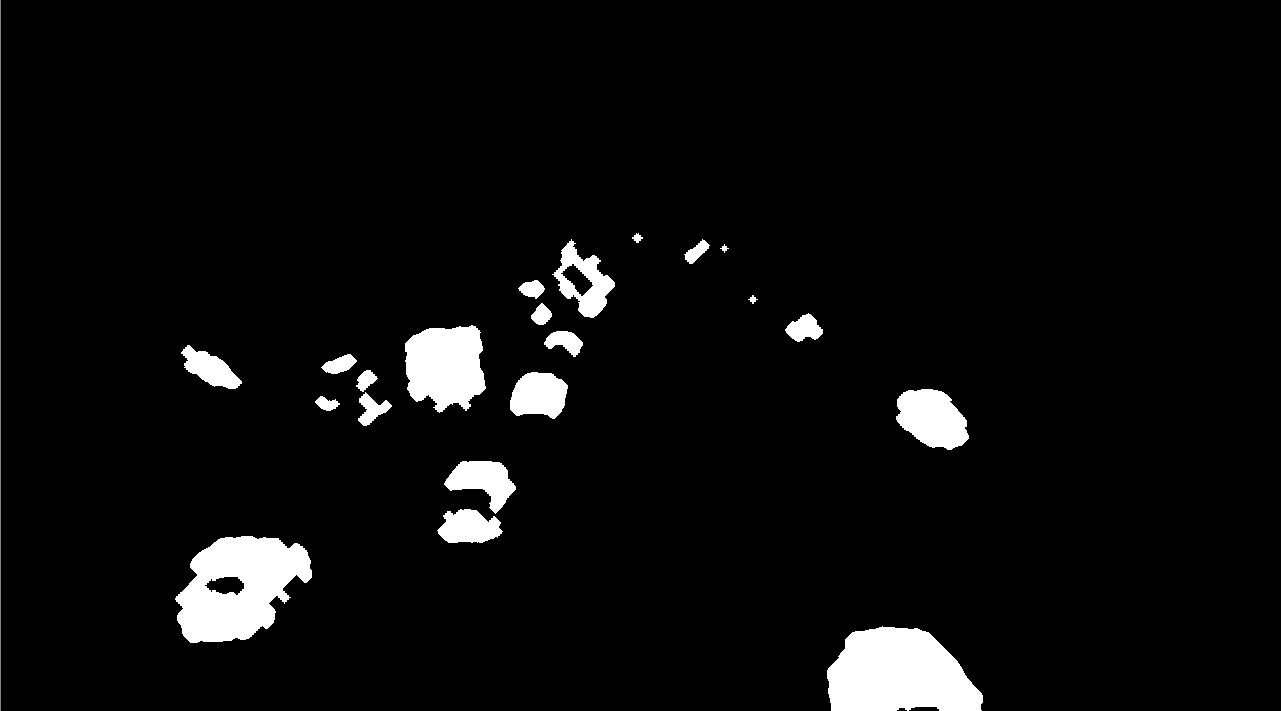
\includegraphics[width=\textwidth]{design/detection/morphology/cross_5}
            % \captionsetup{format = hang}
        \end{subfigure} &
        \begin{subfigure}[b]{0.3\textwidth}
            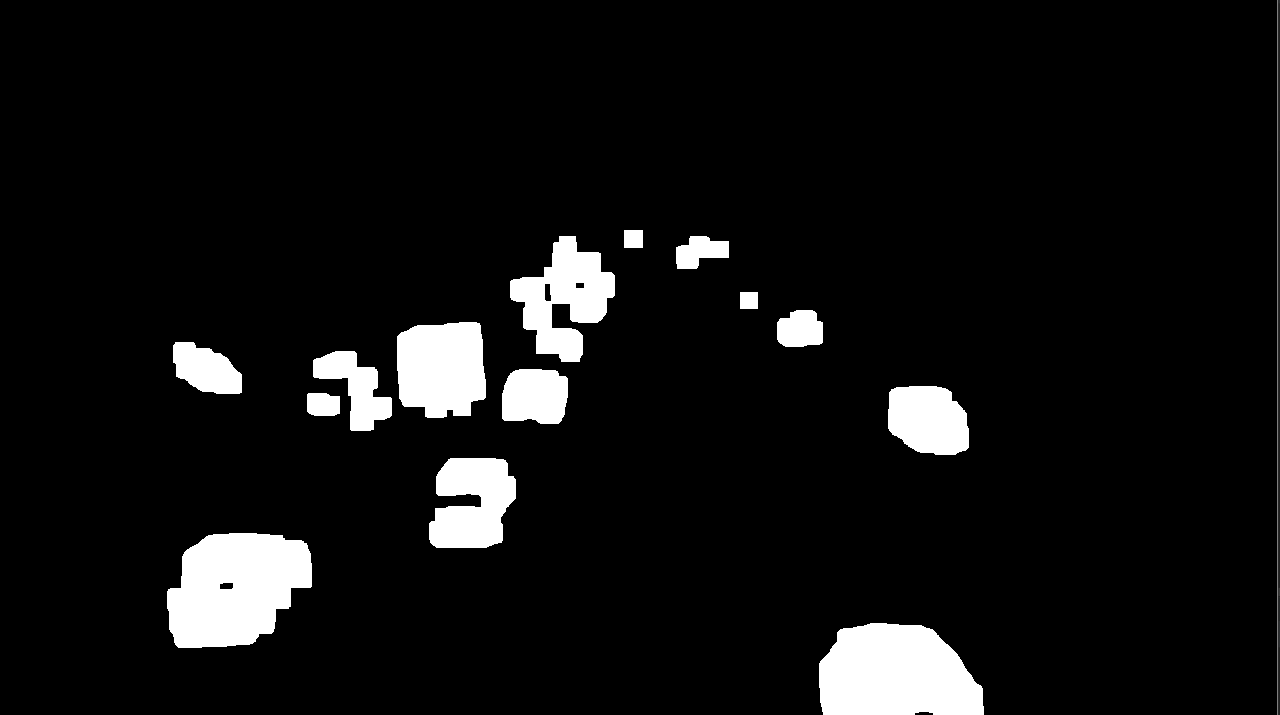
\includegraphics[width=\textwidth]{design/detection/morphology/rect_5}
            % \captionsetup{format = hang}
        \end{subfigure} \\
    \end{tabular}
    \captionsetup{format = hang}
    \caption{Morphological closing using different 7x7 structuring elements and iterations.}
    \label{fig:morph_testing}
\end{figure*}
